%!TEX root = ../thesis.tex

\chapter{The Effect of Lower Mantle Metallization on the Dynamos of Extra-Solar Terrestrial Planets}
\chaptermark{Lower Mantle Metallization in Exoplanets}
\label{chap:superearth}

\section{Introduction}
In our solar system there are seven planets that possess dynamo generated planetary magnetic fields. These planets generate magnetic fields that vary widely in strength and morphology, a difference that reflects the planets varying compositions, thermal histories and internal processes. Given the great diversity of planetary magnetic fields that we observe within our own solar system, a natural assumption to make is that we may have a small and perhaps unrepresentative sample of a larger planetary magnetic field population.

With this in mind, it is worthwhile to consider what types of dynamos may occur in other planetary systems and to consider whether there are any unique  properties that these dynamos possess to aid in their detection. One promising avenue to search for a new class of planetary magnetic field is to first look for planets that have significantly different physical characteristics than planets found in our solar system. One type of planet that appears abundant in other planetary systems that is absent from our own is terrestrial planets with mass greater than that of Earth, more commonly known as ``super-Earth's''. 

\section{Super-Earths}
The most common definition of super-Earths is a predominantly rocky planet with a mass greater than that of Earth. These planets possess much more extreme pressures and temperatures in their interiors than found within the planets of our solar system, allowing for the possibility of exotic material properties and dynamic processes within the planet, potentially affecting magnetic field generation in super-Earths. 

When we plot the distribution of masses from the Open Exoplanet Catalogue \citep{rein2015}. We see that planets with masses larger than Earth appear to be quite common (figure \ref{fig:exoplanetmass}). Figure \ref{fig:exoplanetmass} does not correct for observational biases (large planets, close to their parent star are easier to observe than smaller planets), however \citet{mayor2011harps} finds that after correction, approximately 50 percent of solar-type stars hosts at least one super-Earth or Neptune sized planet.
\begin{figure}
	\centering
        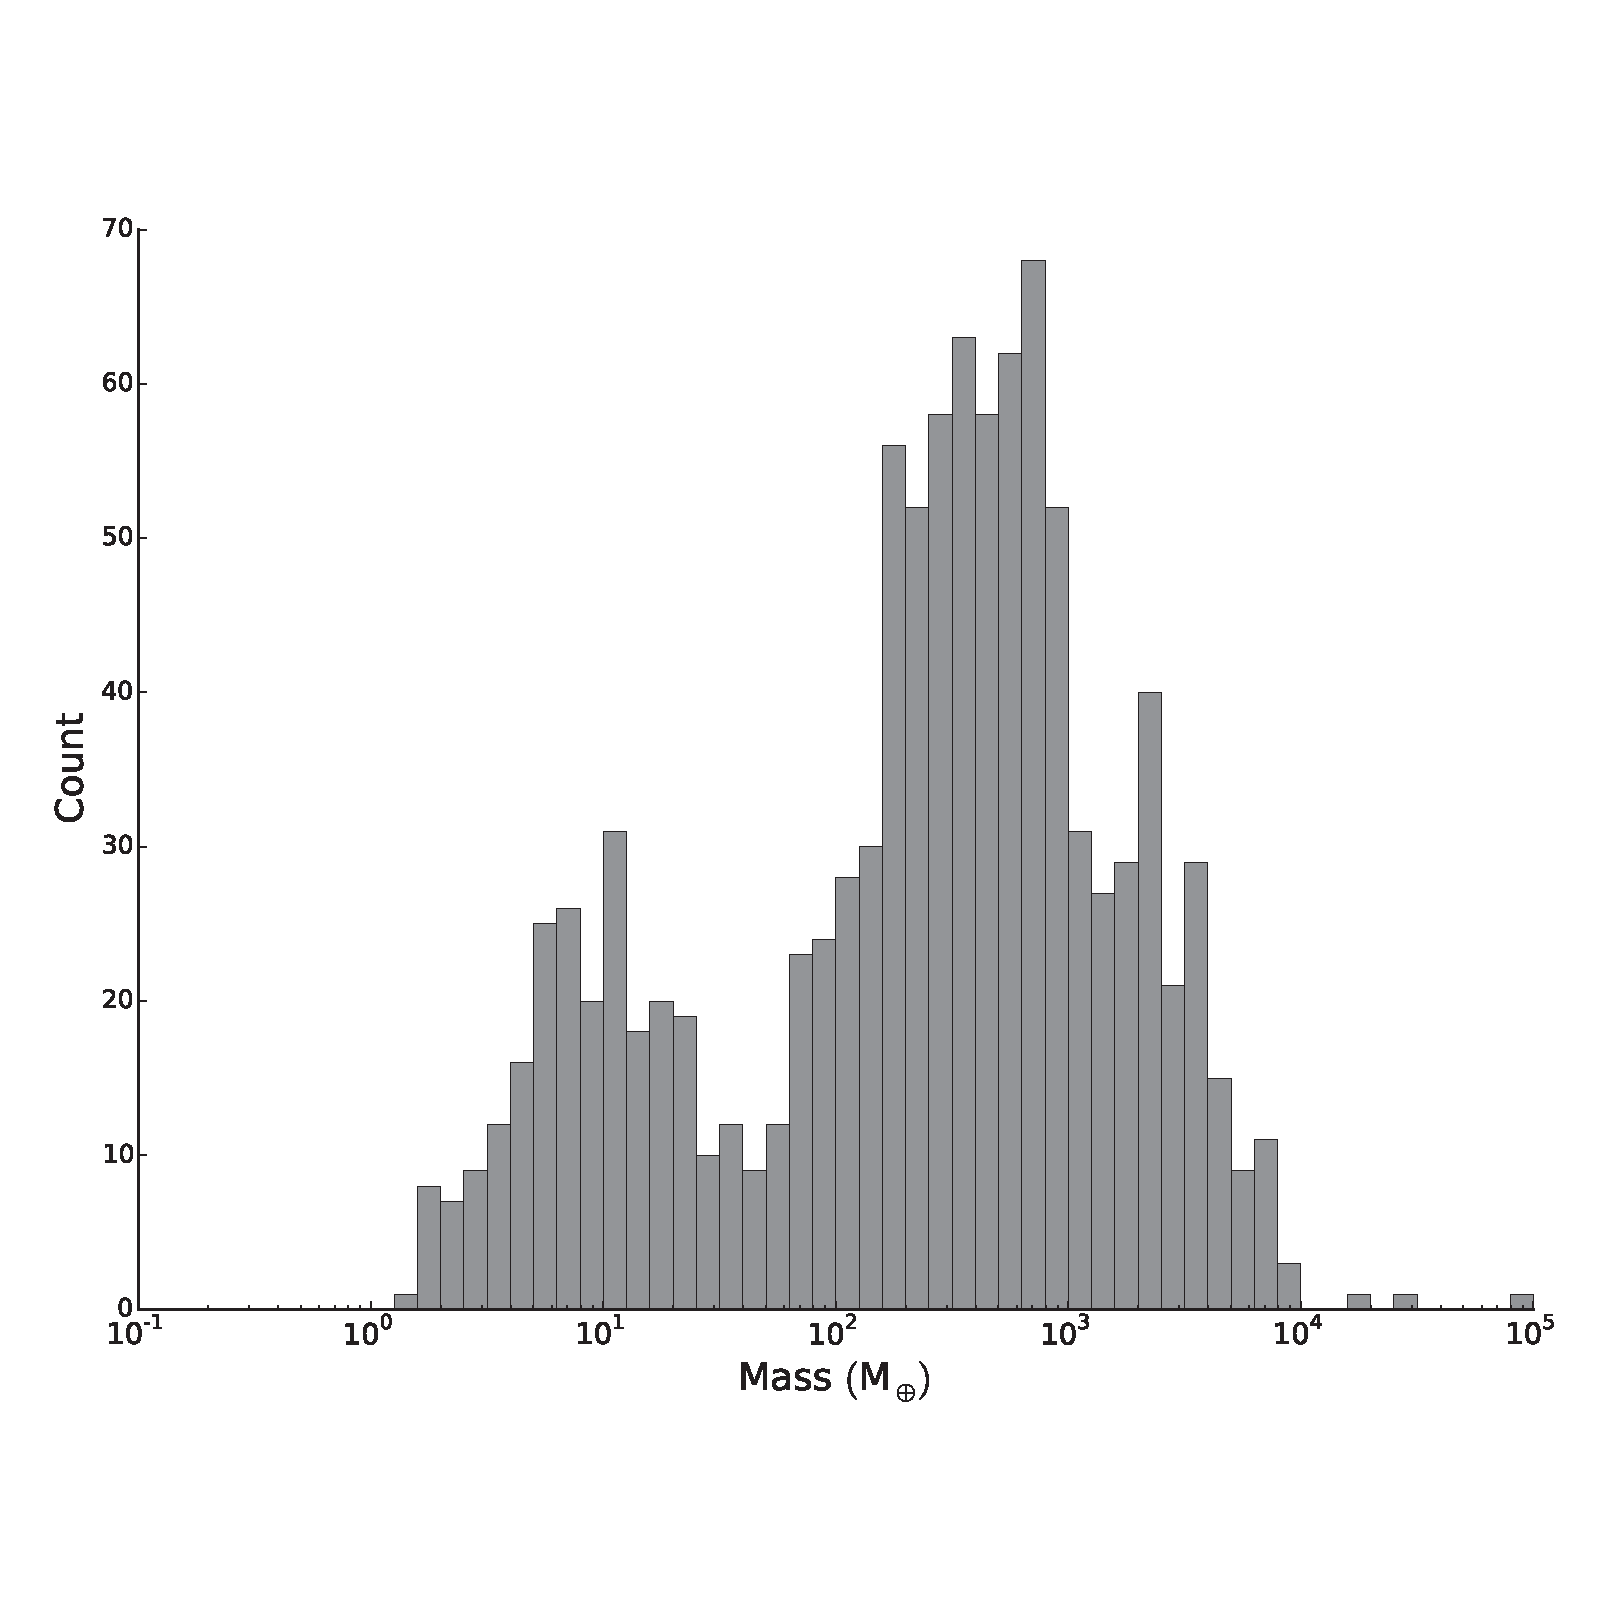
\includegraphics[width=\textwidth]{Chapter3/Figures/ExoplanetsMass.pdf}
        \caption{The distribution of exoplanetary masses for entries in the Open Exoplanet Catalogue \citep{rein2015}}
        \label{fig:exoplanetmass}
\end{figure}

While planets with masses larger than that of Earth seem to be quite common in the sample of observed exoplanets, the mass alone does not imply a composition. In determining composition, the radius of a planet can be a helpful factor as mass and radius combined can give a bulk density. Figure \ref{fig:exoplanetmassradii} shows the mass and radii of 392 planets from the Open Exoplanet Catalogue with measured mass and radii \citep{rein2015}, along with the planets of our solar system, and theoretical mass-radius relations for different bulk compositions. The grey shaded area denotes the region of mass-radius space where super-Earth's are expected to reside.
\begin{figure}
	\centering
        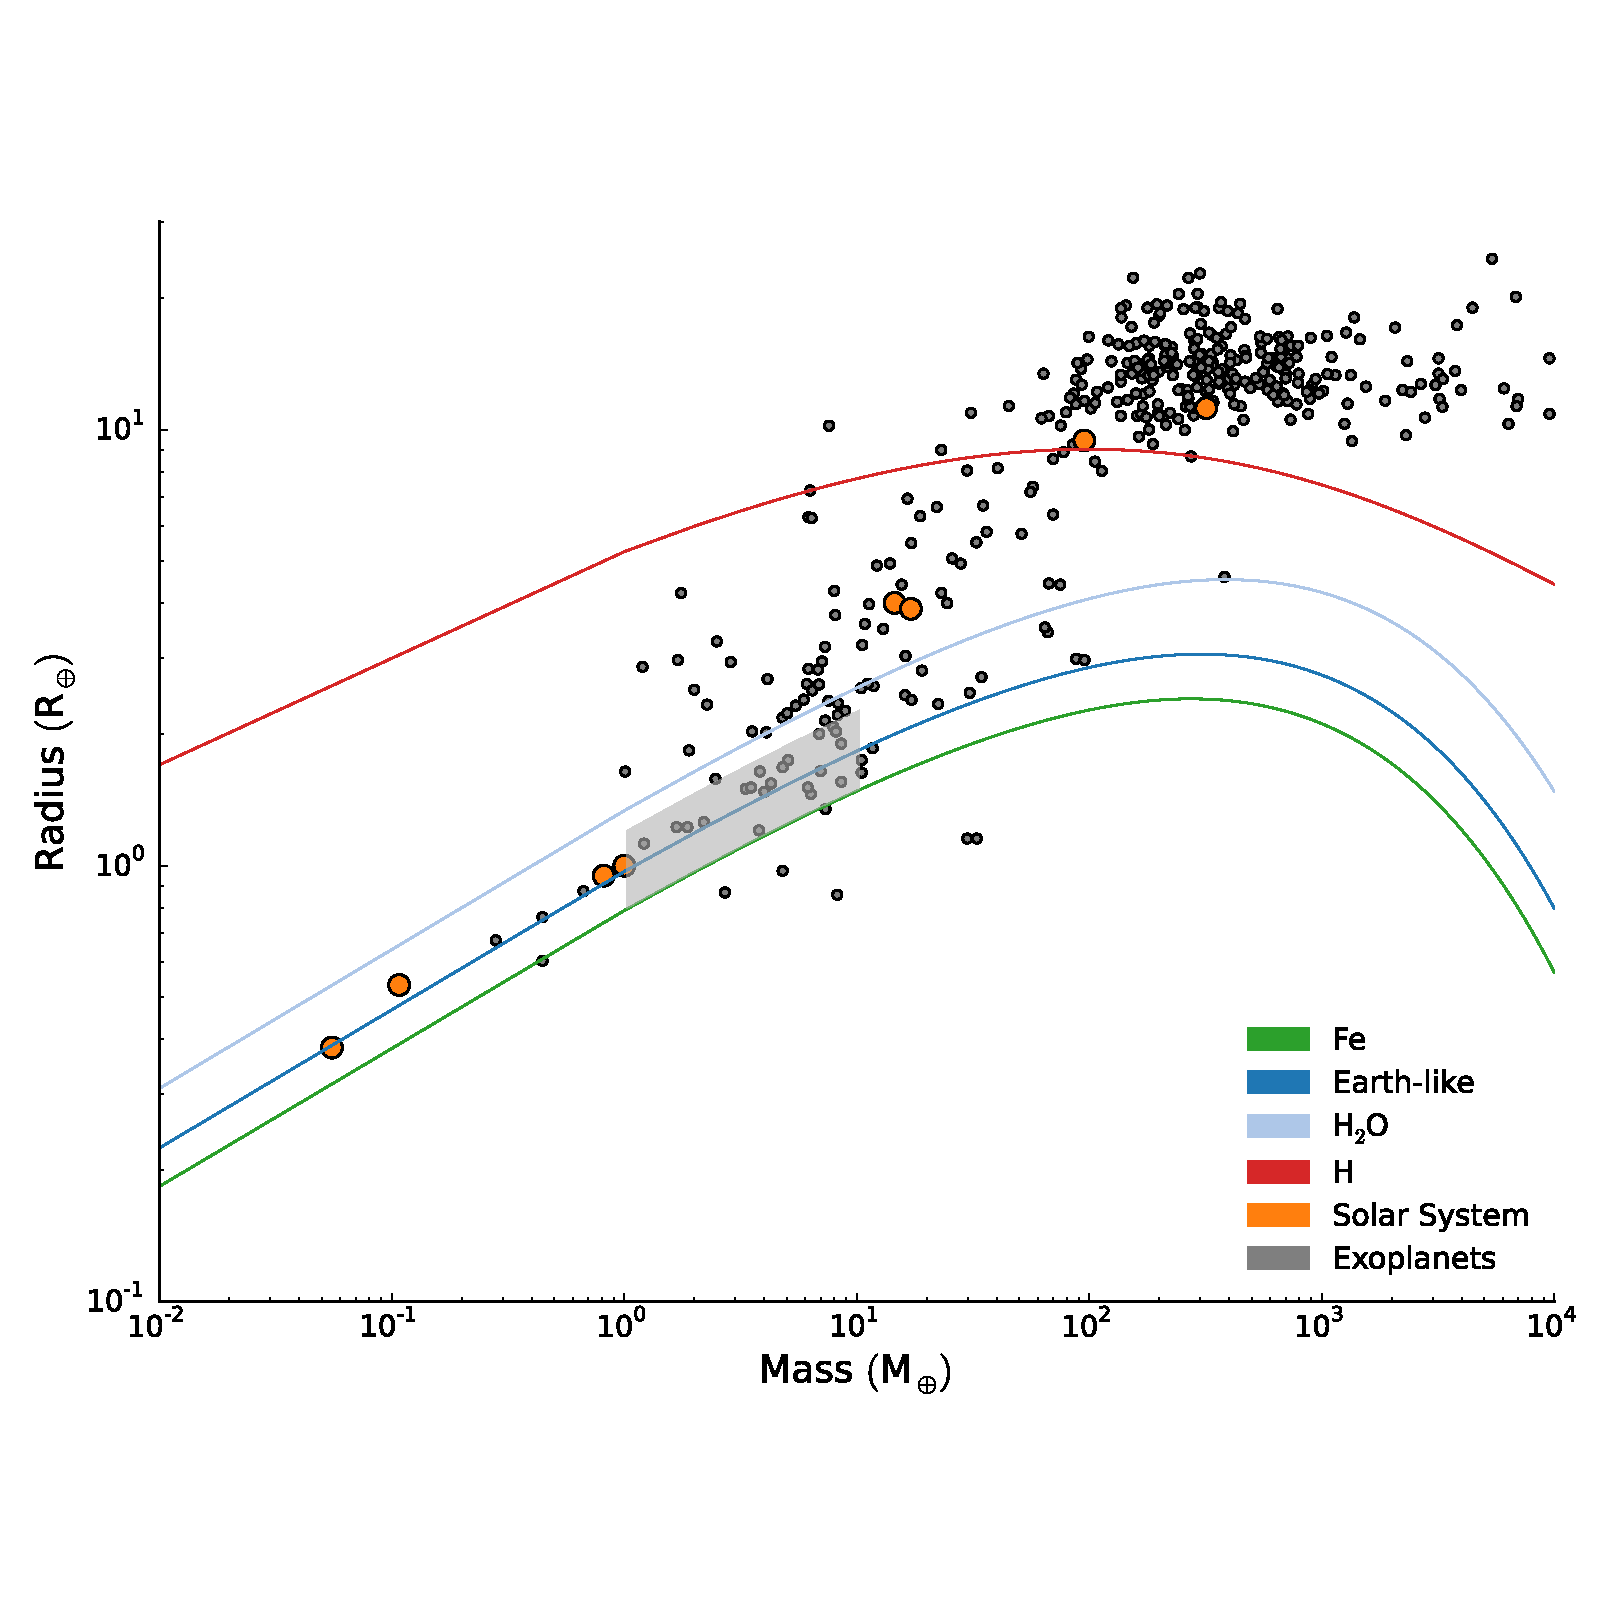
\includegraphics[width=\textwidth]{Chapter3/Figures/ExoplanetsMassRadius.pdf}
        \caption{Planetary radius (in $R_\oplus$) as a function of planetary mass (in $M_\oplus$) for the planets of our solar system (orange circles), the exoplanets in the Open Exoplanet Catalogue with both mass and radius measurements \citep{rein2015} as well as theoretical curves for a pure Fe planet (green), an Earth-like composition ($\textrm{Fe}\left(0.675\right), \textrm{MgSiO}_3(0.325)$, dark blue), a pure $\textrm{H}_{2}\textrm{O}$ planet (light blue) from \citet{seager2007} as well as a pure hydrogen planet (red) from  \citet{zapolsky1969}. The grey shaded region denotes the region of mass-radius space where large terrestrial planets (super-Earth's) should be expected. }
        \label{fig:exoplanetmassradii}
\end{figure}

Figure \ref{fig:exoplanetmassradii} underscores the difficulty of assigning compositions to exoplanets. The lines of constant composition for various combinations of water, ice and rock are very close to each other. When factors such as the uncertainties in both mass and radius, or an atmosphere of unknown mass \citep{adams2008} are added it becomes very difficult to differentiate a large terrestrial planet from a Neptune sized water planet. Nevertheless, the number of planets with mass larger than Earth and radii incompatible with a gaseous composition means that it is likely that super-Earth's are quite common.

\section{Detectability}
Detectability is an important factor in the study of extrasolar planetary magnetic fields. There are two ways that the magnetic field of an extrasolar planet could be detected from Earth. The first occurs when electrons from the stellar wind interact with the dynamo-generated magnetic field from the planet, emitting cyclotron radiation \citep{farrell1999, griessmeier2007, lecacheux1991}. The radiated power associated with this is 
\begin{equation}
P_{rad}\propto B^{0.58} a^{-1.17}
\end{equation}
where $B$ is the magnetic field and $a$ is the planet-star distance. The constant of proportionality is related to the strength of the solar wind \citep{farrell1999}.

The second method by which extrasolar planetary magnetic fields could be detected is through magnetospheric interactions between a close-in planet and its host star. This mechanism was proposed to explain the observations of ``hot spots'' in the chromospheres of some stars, which rotate with the planetary orbit. If a planet with a magnetic field orbits close enough to a star, it is possible the magnetic fields lines may join the two bodies and trap plasma in the closed field lines between them \citep{cohen2009}. The presence of the planetary magnetic field can be detected indirectly through interaction of this plasma with the host star.

Both of these signatures of extrasolar planetary magnetic fields are more easily observable when the magnetic field at the planetary surface is stronger.

\section{Mantle Metallization}
One interesting possibility in super-Earths is the pressure-induced metallization of mantle materials. At high enough pressures, elements which are electrical insulators at ambient or even Earth-mantle pressures will begin to conduct electricity. In order to understand the mechanism behind this, we will briefly discuss the physics of electrical insulators and conductors. More information on the physics of metals and insulators can be found in \citet{ashcroftandmermin}.

\subsection{Band Gaps and Metallization}
If we consider the electronic structure of a solid, we can define two energy ``bands'' that electrons can occupy. The first is the \emph{valence band}, electrons in the valence band are bound to individual atoms and cannot flow between them. The second, at higher electron energy, is the \emph{conduction band}. Electrons in the conduction band are not bound to any atom and can freely flow in response to an applied electric field. Finally, the difference in energy between the lowest energy in the conduction band where the highest energy of the valence band is the \emph{band gap}. In insulators there is a clear separation of energy $E_g$ between the valence band and the conduction band as shown in figure \ref{fig:bandgap}. There are no electrons in the conduction band. In a metal, the band gap is zero, and some electrons occupy the conduction band.
\begin{figure}
	\centering
        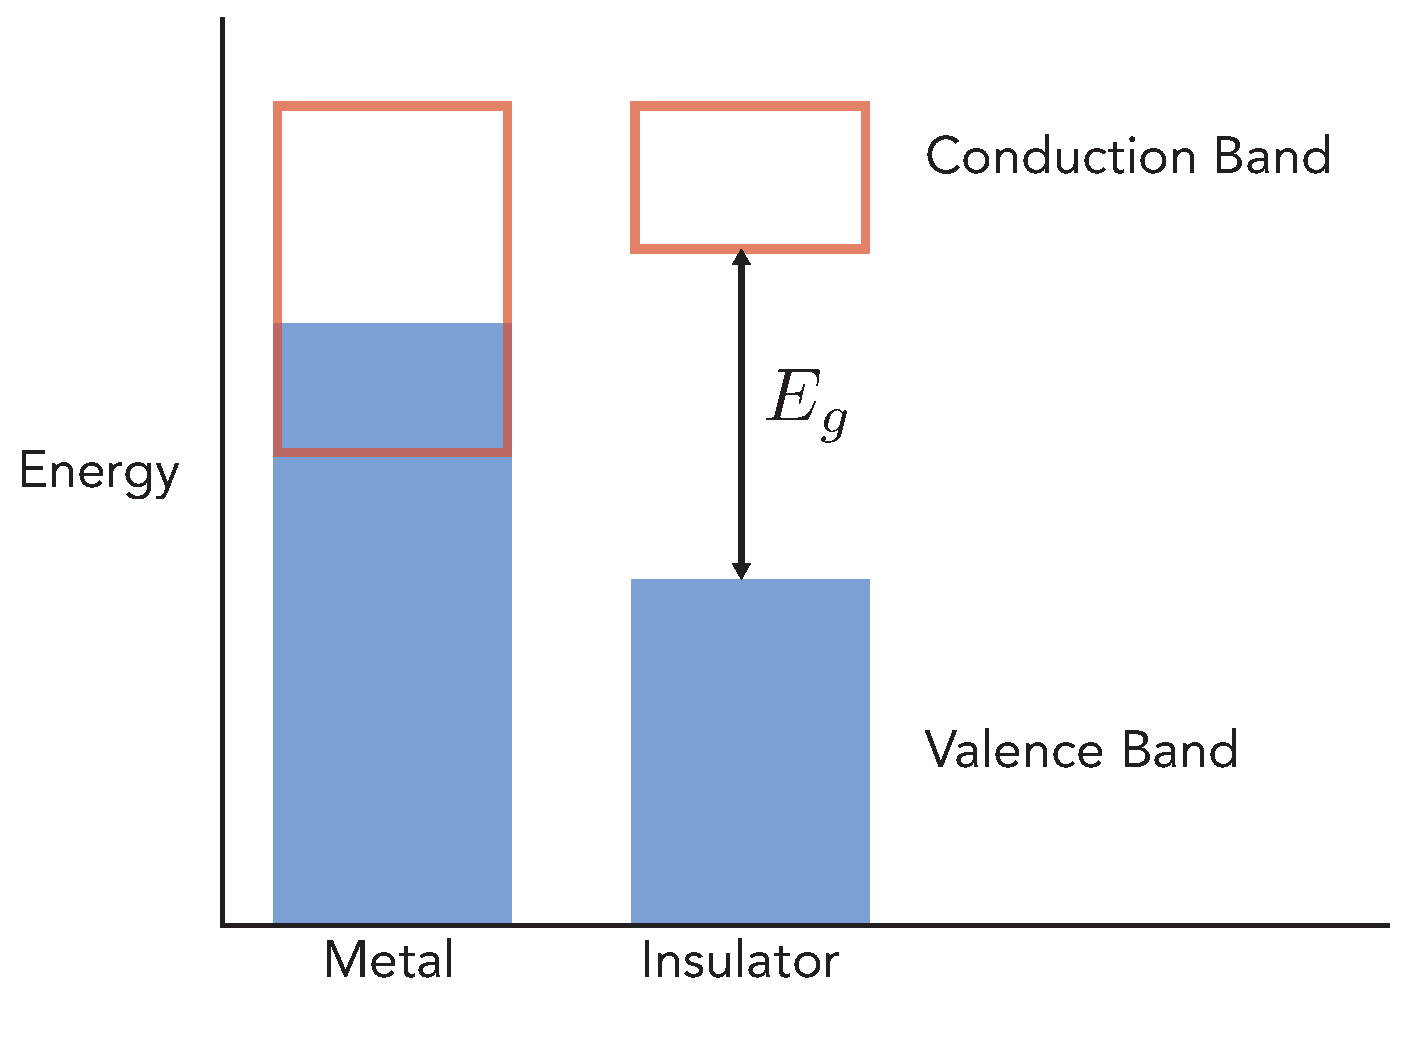
\includegraphics[width=.6\textwidth]{Chapter3/Figures/EnergyGap.eps}
        \caption{A schematic diagram illustrating the difference between the band structure of metals and insulators. Here red indicates the conduction band, and blue indicates the valence band. A filled area indicates that electrons reside at that energy. $E_g$ denotes the band gap.}
        \label{fig:bandgap}
\end{figure}
Importantly, the band gap is pressure dependent, and at high enough pressures it will close, meaning that materials that previously did not conduct electricity become electrical conductors. This process is known as pressure induced metallization.

\subsection{Mantle Metallization in Planets}
In Earth, the mantle is largely electrically insulating, mainly because its main constituent (perovskite) is not expected to metallise until pressures far beyond any which are expected to be found in the deep interiors of even the largest rocky exoplanets \citep{tsuchiya2011}. In exoplanets, the possibility of compositions which differ significantly from Earth could lead to electrically conducting lower mantles in even small rocky exoplanets \citep{ohta2012}. Recent studies have shown that there are several common minerals which should metallise. These include CaSiO$_{3}$ \citep{tsuchiya2011}, FeO \citep{ohta2012}, and Al$_{2}$O$_{3}$ \citep{nellis2010} indicating that lower mantle metallization may be a phenomenon that is common in rocky exoplanets. When mantle materials are metallised a number of their physical properties change significantly. A metallised mantle should have a high thermal conductivity as well as a high electrical conductivity because of the Wiedemann-Franz law, which states that the thermal conductivity is proportional to the electrical conductivity and temperature.

\citet{chan2008} published numerical dynamo simulations with a conducting mantle layer that had  conductivity which varied sinusoidally in latitude and longitude. They found that the addition of this electrically conducting mantle layer could cause a previously steady dynamo to oscillate, and if the conducting mantle layer was thick enough, could stop a dynamo from operating altogether. However, the parameters this study chose were for the benchmark dynamo, an intentionally placid dynamo solution run at unrealistic parameters that is normally used to ensure a numerical dynamo model is working correctly. This raises concerns about its relevance to planetary regimes since the parameters in the benchmark dynamo are much further away from the planetary parameter regime than those used in most planetary studies.

The purposes of these studies was not to model the metallization of the mantle, and so they used lower mantle conductivities than one might expect from a metallic mantle. Furthermore, they concentrated on the effects of heterogeneity in the mantle conductivity. Here we use a numerical dynamo model running at more realistic parameters to study the effect of lower mantle metallization on the dynamos of possible extrasolar terrestrial planets with specific interest in the observable properties of these dynamos.

The study of terrestrial exoplanets, especially terrestrial exoplanetary interiors, remains underconstrained. For a dynamo to exist in these planets, among the most important factors is the state of the mantle. The power  to drive the dynamo of an extrasolar terrestrial planet is controlled by the mantle, so the efficient transfer of heat out of the planet is of great importance. The presence of plate tectonics, and vigorous mantle convection are both efficient ways that planets can drive dynamos in their cores. Currently, mantle convection on these bodies is poorly understood, especially for large exoplanets. The field remains sharply divided \citep{lenardic2012, oneill2007, stein2011, stein2013, valencia2009, vanheck2011} as to the likelihood of plate tectonics, and the viscosity structure \citep{karato2011} of large terrestrial exoplanets. 

The effect of a metallised mantle layer on mantle convection has been studied by \citep{vandenberg2010}. They found that the addition of an electrically conducting layer at the the bottom of the mantle caused the bottom boundary layer to heat, due to the decrease of the local Rayleigh number caused by an increase in the thermal conductivity. This heated lower mantle then becomes buoyant and rises to the upper mantle. This leads to an increased heat flux at the core mantle boundary which could increase the power available to the dynamo, but shorten its lifetime. This would be a secondary effect as the heat flux increase is less than an order of magnitude. There are other, less well constrained properties of extrasolar terrestrial planetary mantles which will have a greater impact on the heat flux from the core than mantle metallization (e.g. radiogenic heating, or the presence of plate tectonics). 

\section{Expected Effects of Mantle Metallization on the Dynamo} 

An electrically conducting mantle should affect the dynamo in two ways. First, any quickly varying components of the magnetic field should be attenuated by the screening effect (see section \ref{sec:screeningderiv}) before they reach the surface, weakening any observed field. Inside the solid mantle layer, the magnetic field obeys a diffusion equation (\ref{eq:nondimmagnetic} with $\mbf{u}=0$), with a diffusivity equal to $\eta=1/(\sigma_{M} \mu_{o})$ where $\sigma_{M}$ is the conductivity of the layer and $\mu_{o}$ is the magnetic permeability of free space. Neglecting the spherical geometry of the core, the magnetic field is attenuated in a solid conducting mantle proportional to $e^{-d\sqrt{\omega/(2 \eta)}}$ where $\omega$ is the frequency of the magnetic field variations at the top of the core and $d$ is the thickness of the conducting mantle. This implies that the thicker the mantle layer, the weaker the observed field. Also, higher multipoles will be preferentially damped due to their more rapid time variation compared to lower multipoles \citep{christensen2004}, while the dipole component of the magnetic field may not be greatly affected.

This screening effect also applies to non-axisymmetric components of the field that are being advected by the background flow at the top of the core. For example, in dynamo simulations, equatorial flux spots are a common occurrence, and typically drift westward \citep{finlay2003}.  From the mantle reference frame these spots are viewed as a time varying magnetic field and hence, they will be screened. In cases where the dynamo generated field is exceptionally steady and axisymmetric, the screening effect may be unimportant as the timescale of field change will be very large.

The second feature we expect when a conducting mantle is added to a dynamo is magnetic shear at the core-mantle boundary (CMB) due to flux freezing in the mantle. The magnetic field should anchor itself in both the solid mantle and the convecting liquid outer core (see \citet{moffatt1978} and section \ref{sec:frozenflux} of this work). Shear should then be created between the solid mantle and the strong zonal flows which are present in planetary cores. Simultaneously, the fluid in the outer core should feel a Lorentz force from the stretching of magnetic field lines anchored in the mantle. While the screening effect is a kinematic process that simply acts on time varying magnetic fields generated by other means, the magnetic coupling effect requires a fully coupled modeling approach.

The thickness of the metallised part of the mantle should have a significant effect on the character of the observable field. We first note that the screening effect and the Lorentz feedback effect scale differently with metallised mantle thickness. Electromagnetic screening becomes more important as the thickness of the metallic mantle layer increases, since the field is attenuated by distance proportional to $e^{-d\sqrt{\omega/(2 \eta)}}$. Conversely, the Lorentz force acting on the fluid by magnetic field anchored in the mantle is nearly independent of mantle thickness. This is evident when examining the equation for the torque ($\Gamma$) on the core by the mantle (adapting \citep{gubbins1987})
\begin{equation}
\Gamma=\frac{r^{2}}{\mu_{o}}\iint\limits_{CMB}B_r\left(\mathbf{r}\mathbf{\mathbf{\times}}\mathbf{B}\right)r^{2} \sin\theta \mathrm{d}\theta \mathrm{d}\phi
\end{equation}
The surface integral is over the core-mantle boundary and does not involve mantle thickness. 

The thickness of the metallised mantle layer in a given exoplanet depends strongly on the size of the planet, the size of the core, and the material which is metallised. For example, FeO should metallise at approximately 55GPa along Earth's geotherm \citep{ohta2012} meaning that a planet significantly smaller than Earth could have an electrically conducting mantle layer as long as it had a large amount of FeO in the mantle. Conversely, CaSiO$_{3}$ is not expected to metallise until pressures of 600GPa, meaning that a conducting mantle layer should form in CaSiO$_{3}$ rich planets with masses greater than 5$M_{Earth}$ \citep{tsuchiya2011}. By varying the composition, planet size, and core size, a conducting mantle layer of nearly any thickness can be achieved. Because of this we avoid fixing a planetary radius or mass, as the arguments here apply equally well to a range of planet sizes. As the surface magnetic field strength is strongly dependent on planetary size and core-mass fraction, we discuss only the properties of the field at the top of the electrically conducting region.
 
\section{Numerical Model}
In this study we use the Kuang-Bloxham numerical dynamo model. We include a solid mantle layer, the electrical conductivity of which can be specified arbitrarily and specify the relative conductivity of the mantle layer with $\sigma_{MC}=\sigma_{M}/\sigma_{C}$ where $\sigma_{M}$ is the conductivity of the conducting mantle layer. All models presented here have $L_{max}=56$, $m_{max}=53$ and the number of grid points in the inner core, outer core, and mantle are $N_{i}=50$, $N_{o}=64$, and $N_{m}=50$ respectively. For numerical reasons we make use of scale-dependent viscosities and diffusivities (hyperdiffusivities, see section \ref{sec:hyperdiffusivity}), we have applied them lightly in this study, using them only for $L>20$ in order to minimise their dynamical effects.

We model a metallised mantle with a spherical shell of uniform conductivity on the outside of the dynamo region. In all models the spherical shell extends from $r_{o}$ to 1.07$r_{o}$. We also make the shell highly conducting, varying $\sigma_{MC}$ from $1/8$ to $1$. As a control, we run a model with a relatively insulating mantle ($\sigma_{MC}=1/400$). A schematic diagram of the model is shown in figure \ref{fig:structure}.
\begin{figure}
\centering
\noindent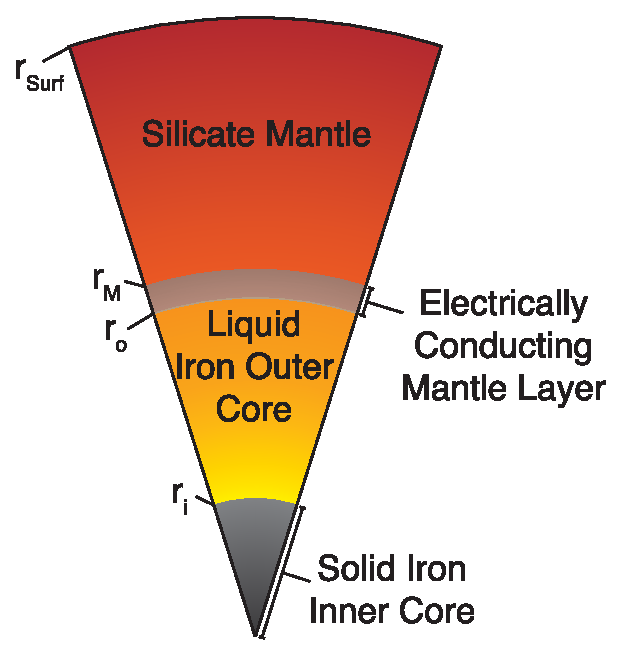
\includegraphics[width=.6\linewidth]{Chapter3/Figures/f1.eps}
\caption{A schematic diagram of the structure of a planet with a conducting mantle layer. Our numerical model solves in the region below $r_{M}$.}
\label{fig:structure}
\end{figure}

The strong rotational influence on convection in planetary cores implies that the solid inner core has a significant effect on the dynamo \citep{heimpelandaurnou2005, stanleyfluxspot}. Since exoplanets can be found in  different stages of their thermal evolution (depending on their age), we use three different inner core sizes in this study. As a planet ages, the heat lost from the core will cause the solid inner core to grow, so the different cases can be considered proxies for different stages of the life of the dynamo. Here we use $r_{io}=0.35$, $0.5$, and $0.70$. The electrical conductivity of the inner core is the same as the fluid outer core, and the inner core is allowed to rotate independently of the outer core and the mantle in three dimensions in response to viscous and electromagnetic torques exerted on it by the fluid outer core.

\section{Results}
In all cases we find that the addition of an electrically conducting mantle significantly enhances magnetic field generation in our models. The most striking example of this is in the axisymmetric azimuthal ($\phi$) component of the field near the core-mantle boundary (figure \ref{fig:toroidal}).
\begin{figure}
\centering \noindent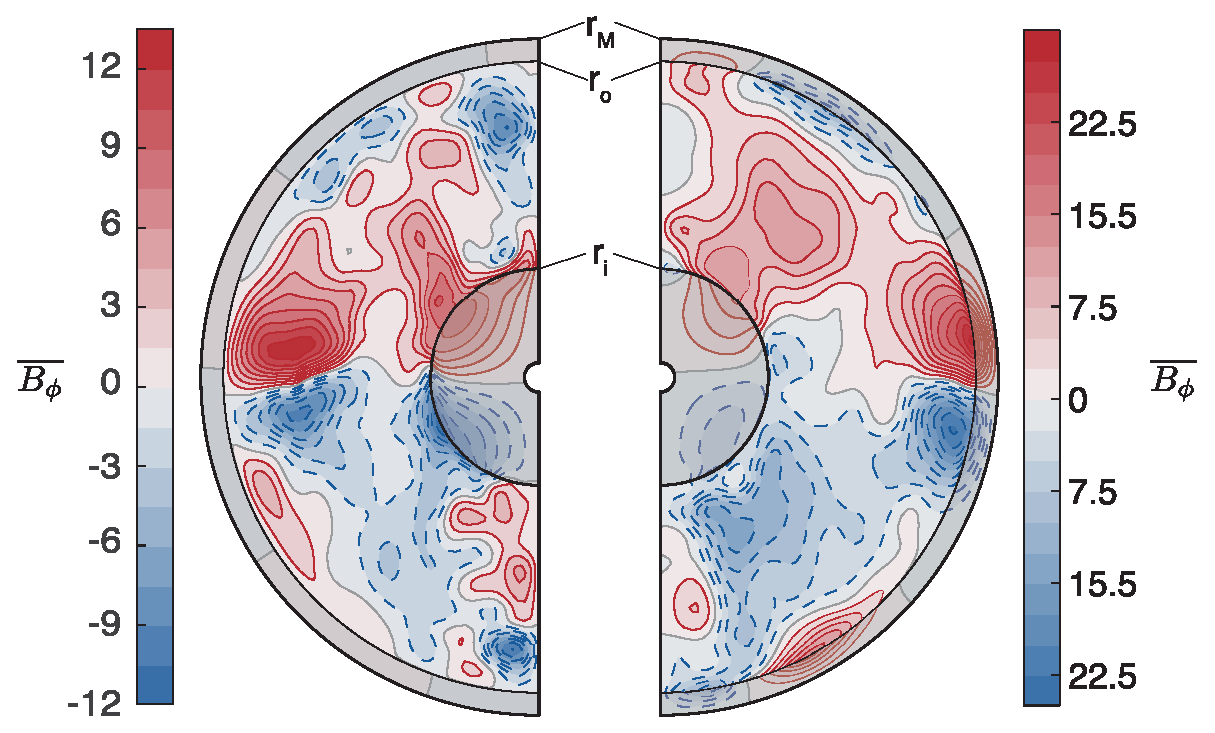
\includegraphics[width=.8\linewidth]{Chapter3/Figures/f2.eps}
\caption{Contours of the axisymmetric azimuthal ($\phi$) component of the magnetic field for an insulating mantle ($\sigma_{MC}=1/400$, left) and for a conducting mantle ($\sigma_{MC}=1$, right) at a single moment in time. The shaded regions indicate the inner core (center) and the conducting mantle layer (outside). Note the difference in scales between the two plots. In these models $r_{io}=0.35$.}
\label{fig:toroidal}
\end{figure}
Here magnetic fields anchored in both the solid, stationary mantle, and the fluid outer core are sheared by the strong zonal flows at the top of the core. This provides a source of magnetic field stretching, which strengthens the magnetic field in the azimuthal direction.

We find that the strength of the poloidal component of the field at the core-mantle boundary is increased as well (figure \ref{fig:cmbenergies35}-\ref{fig:cmbenergies70}).
\begin{figure}
	\centering
        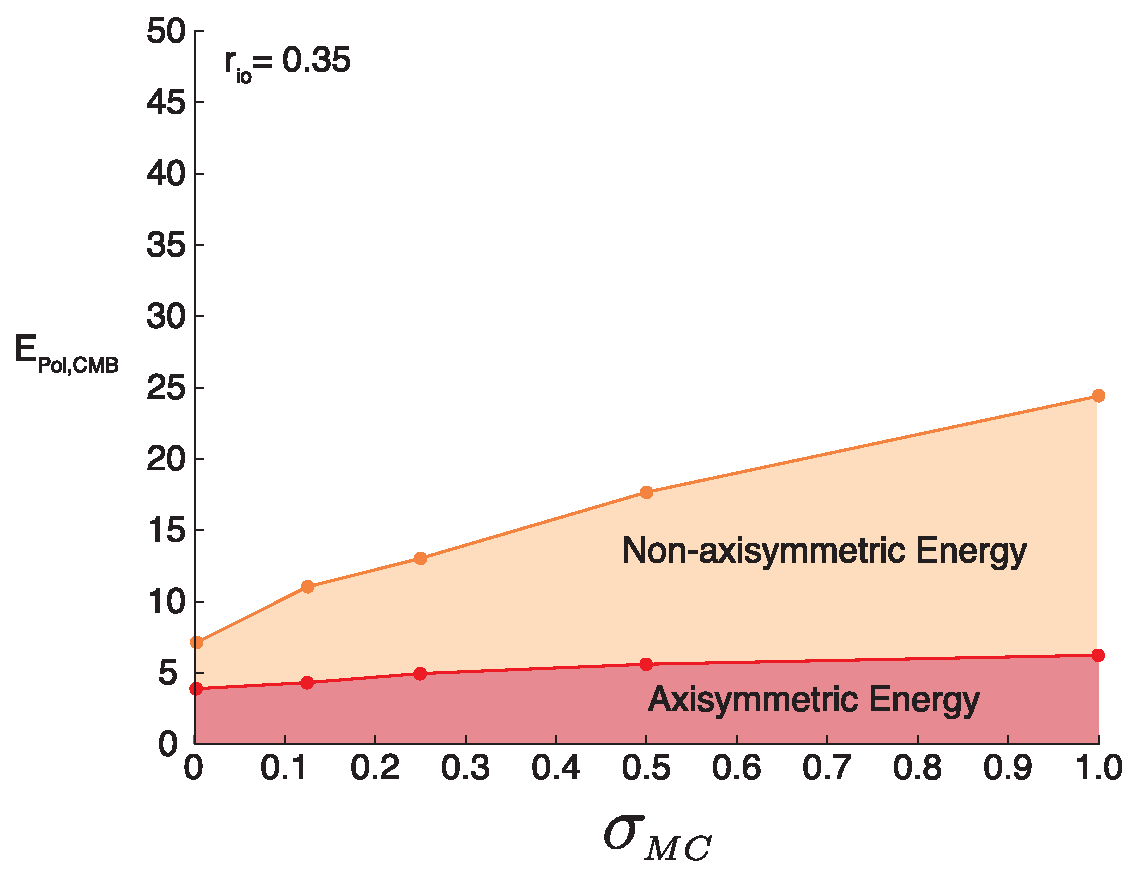
\includegraphics[width=.7\textwidth]{Chapter3/Figures/f3a.eps}
        \caption{The poloidal energies at the core-mantle boundary for $r_{io}=0.35$ separated into non-axisymmetric components (upper) and axisymmetric components (lower). All points are a time average over at least one magnetic diffusion time.}
        \label{fig:cmbenergies35}
\end{figure}
\begin{figure}
	\centering
        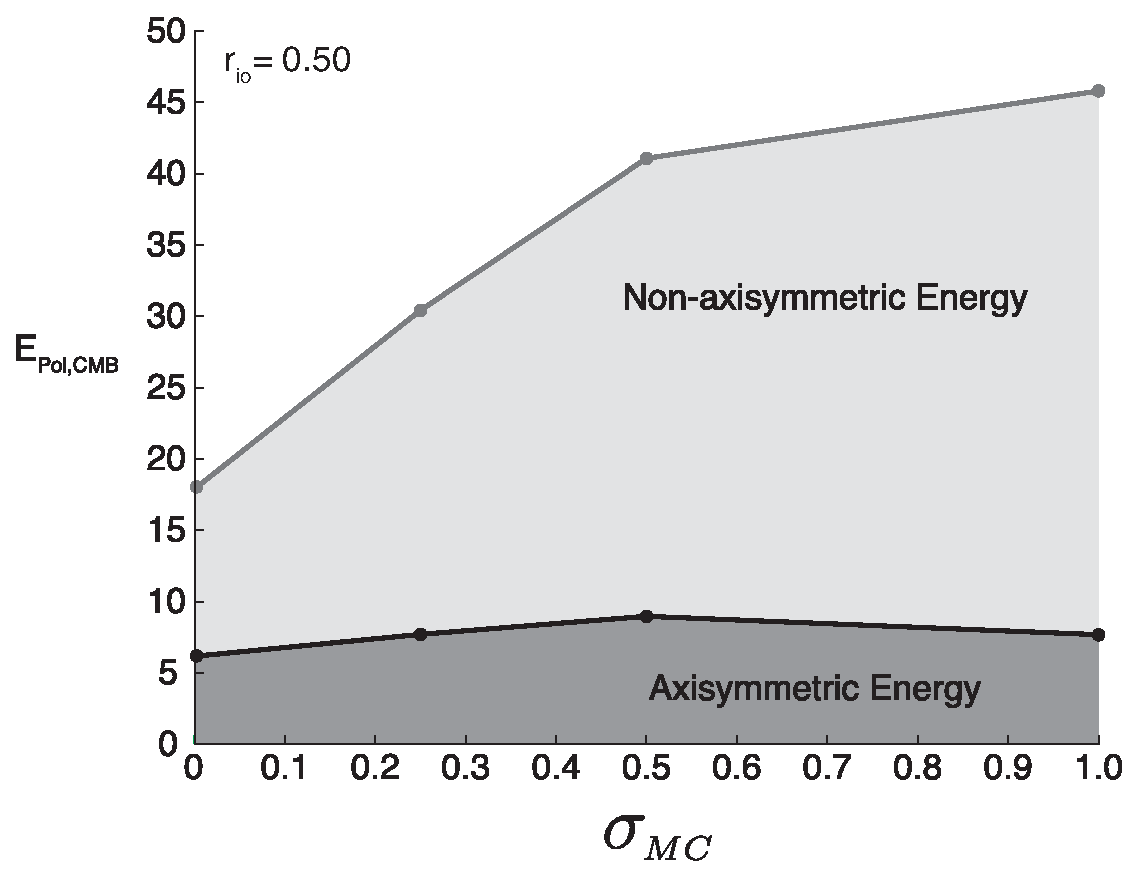
\includegraphics[width=.7\textwidth]{Chapter3/Figures/f3b.eps}
        \caption{The poloidal energies at the core-mantle boundary for $r_{io}=0.50$ separated into non-axisymmetric components (upper) and axisymmetric components (lower). All points are a time average over at least one magnetic diffusion time.}
        \label{fig:cmbenergies50}
\end{figure}
\begin{figure}
	\centering
        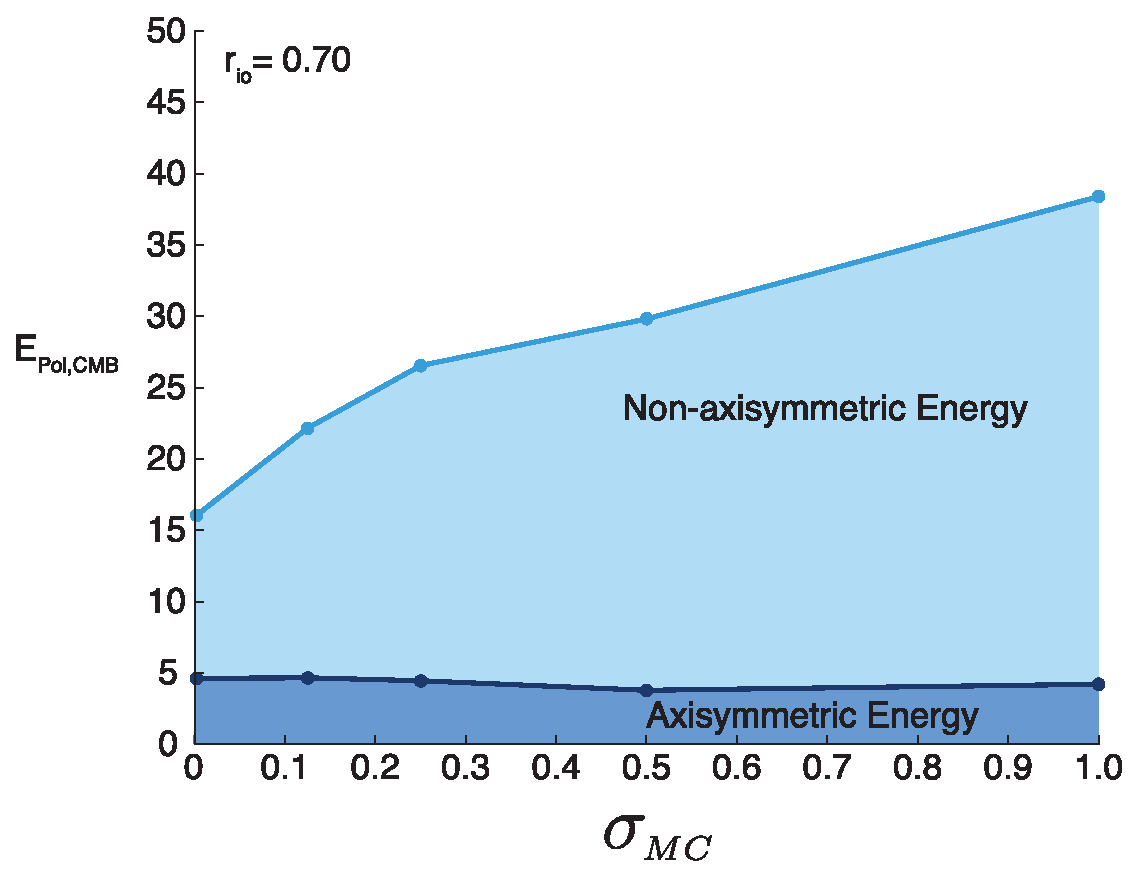
\includegraphics[width=.7\textwidth]{Chapter3/Figures/f3c.eps}
        \caption{The poloidal energies at the core-mantle boundary for $r_{io}=0.70$ separated into non-axisymmetric components (upper) and axisymmetric components (lower). All points are a time average over at least one magnetic diffusion time.}
        \label{fig:cmbenergies70}
\end{figure}

The poloidal component of the field is of special interest as it is the component which is observable from outside the conducting region (the toroidal field requires poloidal currents, which are only present in the conducting region). In our models, the energy in the non-axisymmetric component of the poloidal field increases as the conductivity of the mantle layer increases. In all cases the energy in the axisymmetric component of the poloidal field remains approximately constant.

This preferential increase in the non-axisymmetric component of the field can be explained by noting that the toroidal field at the core-mantle boundary is predominantly axisymmetric, due to the large zonal axisymmetric flows shearing magnetic field there. Given this we can use the Bullard-Gellman formalism (\citet{bullard1954} and Appendix \ref{chap:appendix1}) to show that a dynamo cannot create axisymmetric poloidal energy by any flows acting on axisymmetric toroidal magnetic fields.

In the notation of the Bullard-Gellman formalism, the situation of creating axisymmetric poloidal magnetic field from axisymmetric toroidal magnetic field can be represented as
\begin{equation}
T_{\alpha}^{m_{\alpha}} T_{\beta}^{0} P_{\gamma}^{0} +P_{\alpha}^{m_{\alpha}} T_{\beta}^{0} P_{\gamma}^{0}.
\end{equation}
Recall that $T$ and $P$ represent the toroidal and poloidal fields respectively, $\alpha$ and $m_\alpha$ represent the velocity field spherical harmonic mode, $\beta$ and $m_\beta$ represents the seed magnetic field mode, and $\gamma$ and $m_\gamma$ represents the resultant magnetic field spherical harmonic mode. In this case we include all possible modes of the velocity field, and axisymmetric modes of the seed and magnetic field. 

Evaluating these terms is quite straight forward. The $T_{\alpha}^{m_{\alpha}} T_{\beta}^{0} P_{\gamma}^{0}$ interaction is always identically zero, it merely states that toroidal flows acting on toroidal magnetic fields cannot produce poloidal fields, a well known ``anti-dynamo'' theorem. The $P_{\alpha}^{m_{\alpha}} T_{\beta}^{0} P_{\gamma}^{0}$ interaction requires the selection rules outlined in Appendix \ref{chap:appendix1} to evaluate. Terms of this type depend on an Elsasser integral:
\begin{equation}
L=\oint_{S}Y_{\gamma}^{m_{\gamma}*}\left(\frac{\partial Y_{\alpha}^{m_\alpha}}{\partial \theta}\frac{\partial Y_{\beta}^{m_\beta}}{\partial \phi}-\frac{\partial Y_{\alpha}^{m_\alpha}}{\partial \phi}\frac{\partial Y_{\beta}^{m_\beta}}{\partial \theta}\right)dS.
\end{equation}
This is zero due to a confluence of two of the selection rules for Elsasser integrals. First, in order to be non-zero $m_\alpha\pm m_\beta \pm m_\gamma =0$, implying that $m_\alpha=0$. A second requirement for Elsasser type integral to be non-zero is that either two or none of the harmonics has a $\cos\left(m\phi\right)$ term ($m=0$ is a cosine term here). Since all three of our harmonics have $m=0$ we have three cosine terms, meaning the $P_{\alpha}^{m_{\alpha}} T_{\beta}^{0} P_{\gamma}^{0}$ is always zero. Hence, we should expect that the axisymmetric poloidal field should not increase due to an increase in the axisymmetric toroidal field caused by a conducting mantle layer. This application of the selection rules only applies to cases where $m=0$ for all three modes. It is possible to create non-axisymmetric poloidal fields via non-axisymmetric velocities acting on axisymmetric toroidal magnetic fields, so an increase in the strength of the axisymmetric toroidal magnetic field should imply an increase in the strength of the non-axisymmetric poloidal magnetic field. 

The axisymmetry of a dynamo is an important factor in the potential observability of extrasolar terrestrial planetary magnetic fields. For the magnetic field to reach the exterior of the planet where it can be observed, it must first be screened through a conducting lower mantle. As  discussed earlier, non-axisymmetric fields are screened more efficiently than axisymmetric fields. This becomes apparent if we plot the poloidal magnetic energies above the conducting layer (figure \ref{fig:ddppoloidaltotal}).
\begin{figure}
\noindent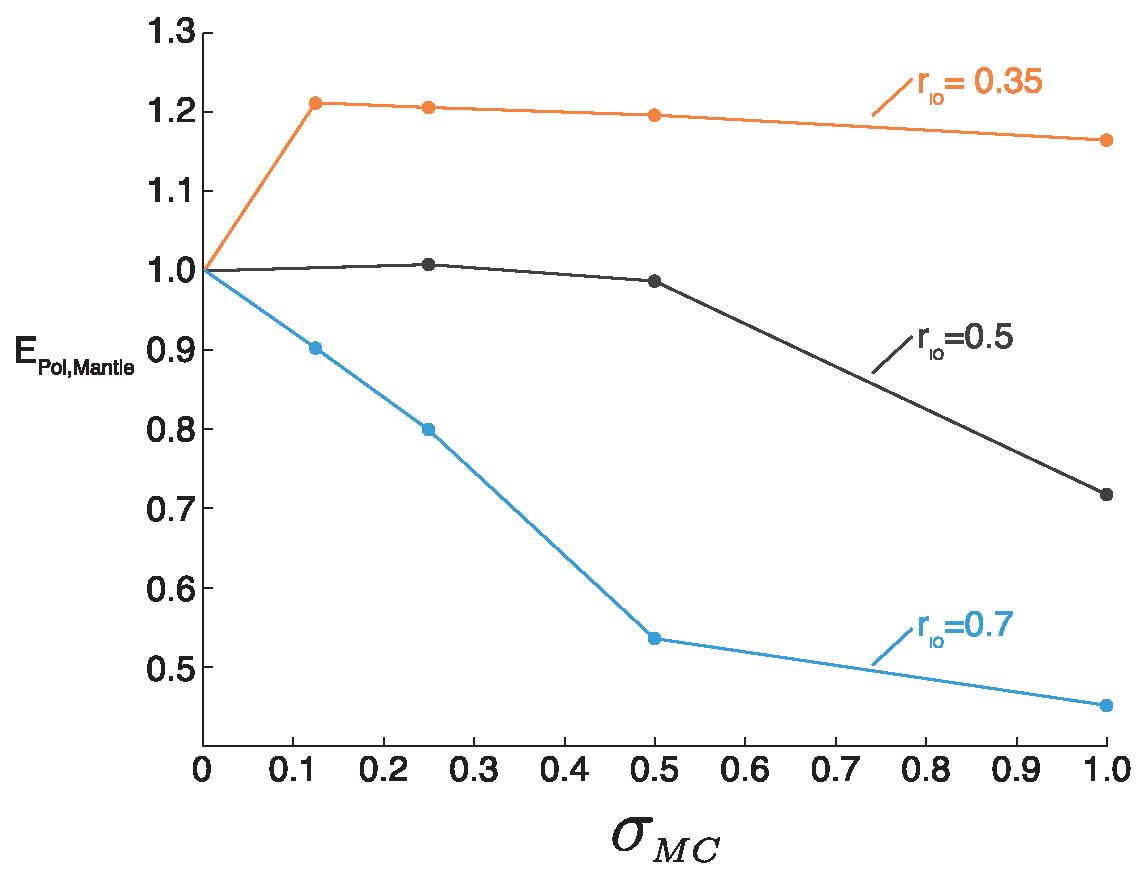
\includegraphics[width=.7\linewidth]{Chapter3/Figures/f4.eps}
\centering
\caption{Total poloidal energy at the top of the conducting layer ($r_{M}$) as a function of mantle conductivity. All points are a time average over at least one magnetic diffusion time and have been normalised to the insulating mantle case.}
\label{fig:ddppoloidaltotal}
\end{figure}
We see that depending on the inner core size, the observable field is either only marginally stronger, or much weaker than the field in a model without a conducting mantle layer.

As $r_{io}$ increases there is a marked decrease in poloidal field strength at the top of the conducting layer relative to the insulating case (figure \ref{fig:ddppoloidaltotal}). When considered with figures \ref{fig:cmbenergies35}-\ref{fig:cmbenergies70}, the reason for this becomes clear. As the liquid outer core becomes thinner the dynamo becomes less axisymmetric at the top of the dynamo region and the characteristic timescale of variation becomes shorter \citep{aubert2009}. Both of these effects cause the field to be weakened by the screening effect of the conducting layer. This means thinner shells are more susceptible to the screening effect discussed earlier. The increase in non-axisymmetry with increasing $r_{io}$ has been observed previously in studies which modelled the evolution of Earth's dynamo through time \citep{aubert2009, roberts2001}.

\section{Conclusions}

We have used a numerical planetary dynamo model to investigate the effect of the metallization of silicate mantles on the observable magnetic fields of super-Earths. We have carried out models for three different inner core sizes to simulate these planets at different stages in their thermal evolution. In all cases we find that the strength of the internal magnetic field increases substantially, owing to the magnetic shear provided at the core-mantle boundary by the conducting mantle. We also find that the addition of a conducting mantle makes the field significantly less axisymmetric at the top of the dynamo region. After being screened through the conducting mantle layer we find that the observable field shows either a modest increase in field strength (at $r_{io}=0.35$) or a significant decrease in field strength (at $r_{io}=0.7$). The results of this work are published in \citet{vilim2013}

As we have used a thin conducting layer in these models (compared to the range that is possible for terrestrial exoplanets), we expect that in larger planets, the screening effect would be even stronger than we observe here. This means that any planets with a metallised mantle should have surface fields which have been significantly weakened by a combination of the non-axisymmetrisation of the dynamo, and the screening effect of the mantle. We therefore expect that the metallization of silicates should make the detection of dynamo-generated magnetic fields from super-Earth's more difficult than previously anticipated \citep{driscoll2011}.









